\subsection{Analisis Alternatif Solusi}
\label{subsec:analisis-alternatif-solusi}

\subsubsection{Pendekatan Solusi}
Berdasarkan analisis masalah pada bagian \ref{subsec:analisis-masalah}, terdapat beberapa kebutuhan yang perlu dipenuhi dalam pengembangan solusi. Pemenuhan kebutuhan-kebutuhan ini akan menjadi konsiderasi untuk memilih alternatif solusi yang tepat. Altenatif-alternatif solusi akan dibagi menjadi beberapa kategori berdasarkan kebutuhan yang dipenuhinya, yaitu:

\begin{enumerate}
	\item Ekstraksi data Smart Contracts dari Blockchain Ethereum
	\item Pemodelan, penyimpanan, dan \textit{indexing} data Smart Contracts
	\item Klasifikasi fungsional dan semantik Smart Contracts
	\item Pencarian dan rekomendasi Smart Contracts berdasarkan kebutuhan pengguna dan pengembang
\end{enumerate}

Selain keempat alternatif tersebut, akan digunakan GUI dan API bagi pengguna untuk mengakses sistem.

Bagian berikut akan menguraikan alternatif yang memenuhi tiap kebutuhan. Alternatif yang disajikan berasal dari peninjauan sejumlah riset relevan, berfungsi sebagai referensi sekaligus fondasi pengembangan solusi. Peninjauan ini mempertimbangkan aspek seperti aksesibilitas hasil riset, kompleksitas teknis, skalabilitas, dan dukungan fungsional.

\subsubsection{Ekstraksi Data Smart Contracts dari Blockchain Ethereum}

\begin{figure}[ht]
	\centering
	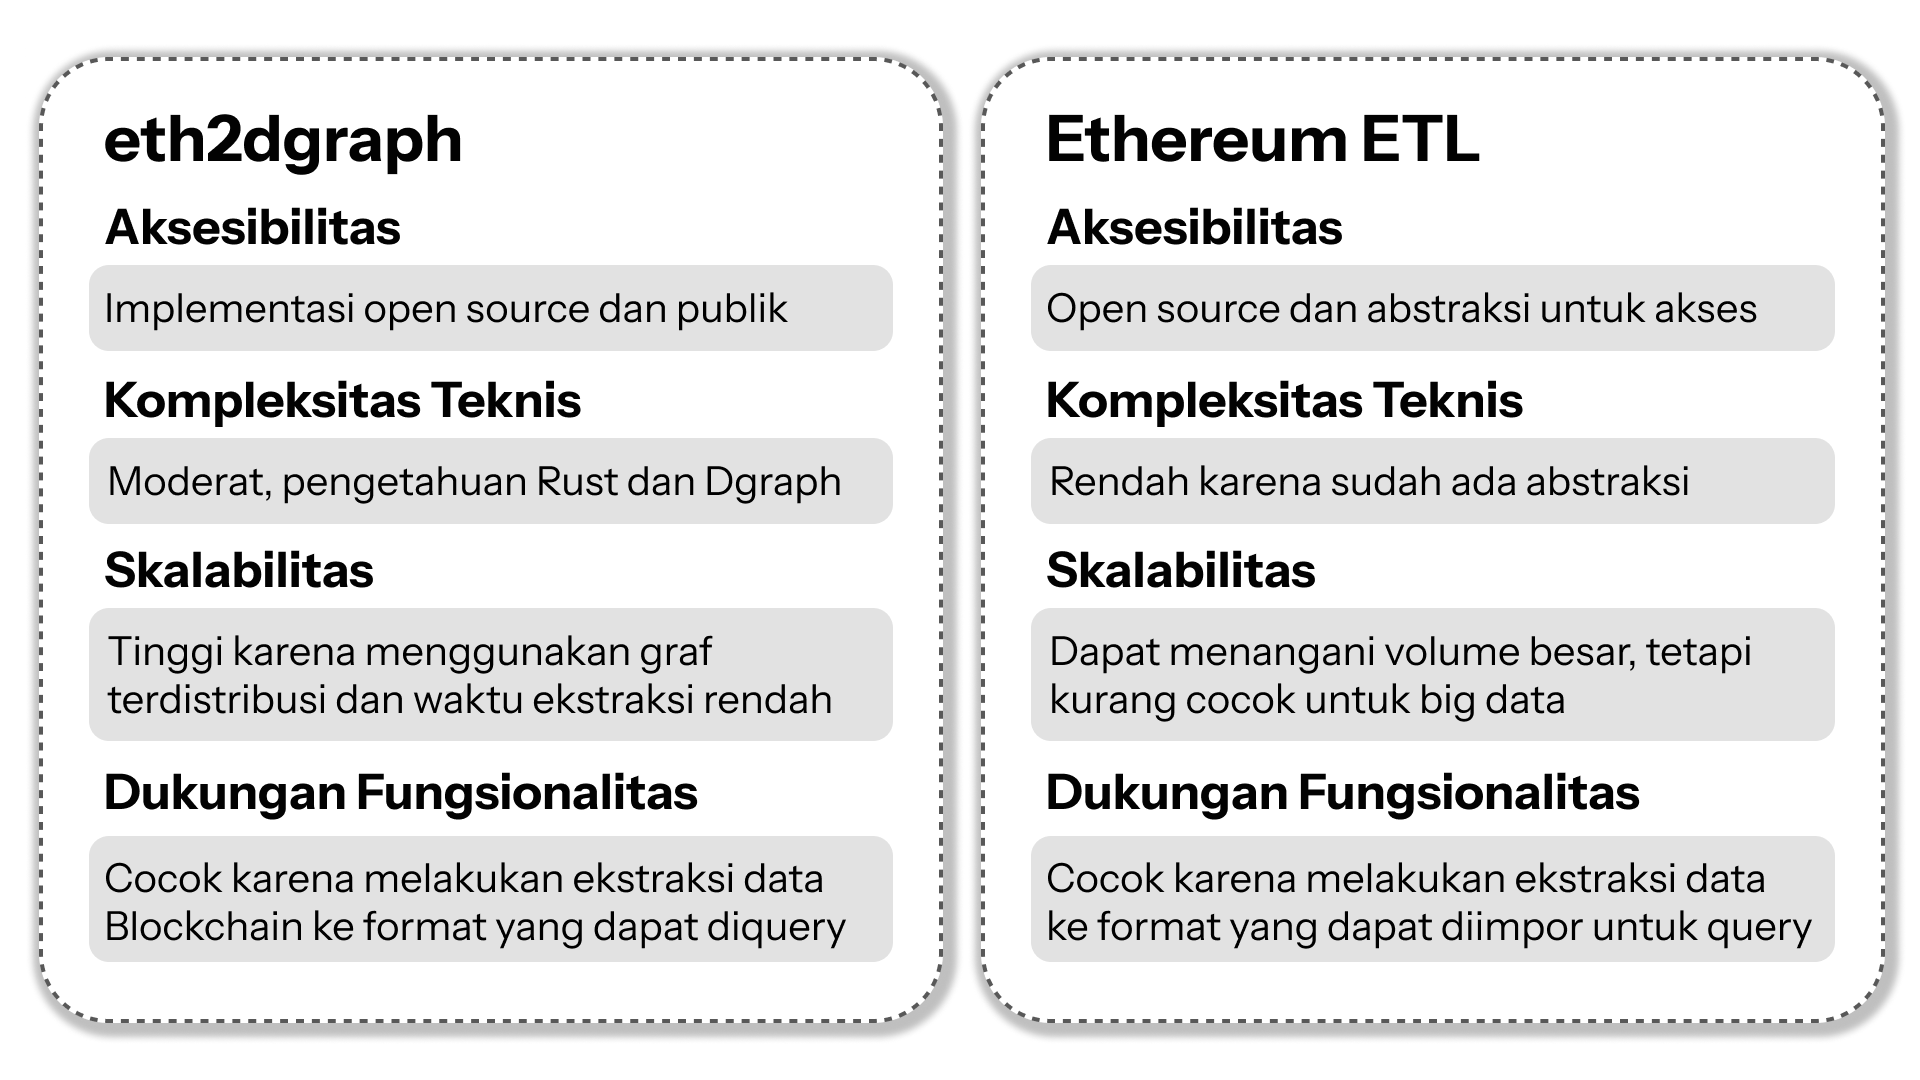
\includegraphics[width=0.9\textwidth]{resources/chapter-3/ekstraksi-1.png}
	\caption{Perbandingan alternatif ekstraksi data Smart Contracts dari Blockchain Ethereum}
	\label{image:perbandingan-ekstraksi-1}
\end{figure}

\begin{figure}[ht]
	\centering
	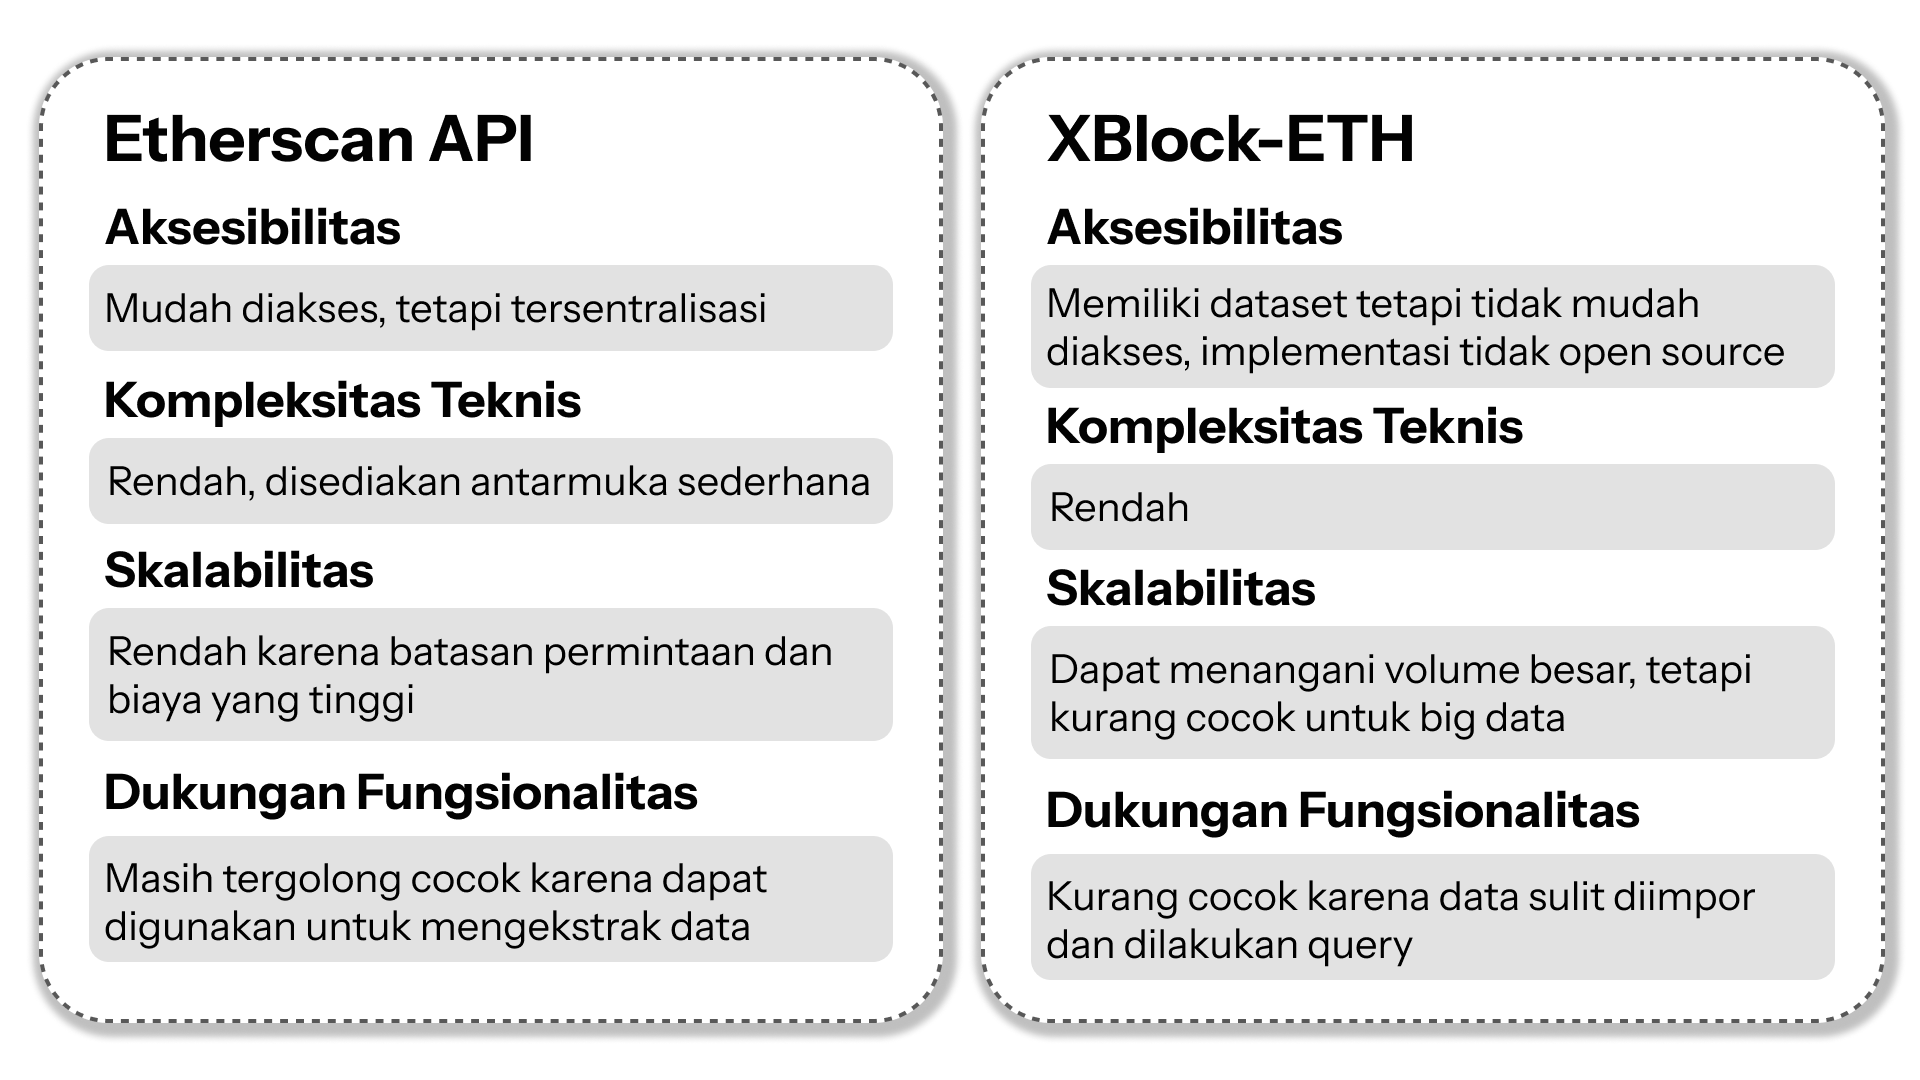
\includegraphics[width=0.9\textwidth]{resources/chapter-3/ekstraksi-2.png}
	\caption{Perbandingan alternatif ekstraksi data Smart Contracts dari Blockchain Ethereum}
	\label{image:perbandingan-ekstraksi-2}
\end{figure}

\begin{figure}[ht]
	\centering
	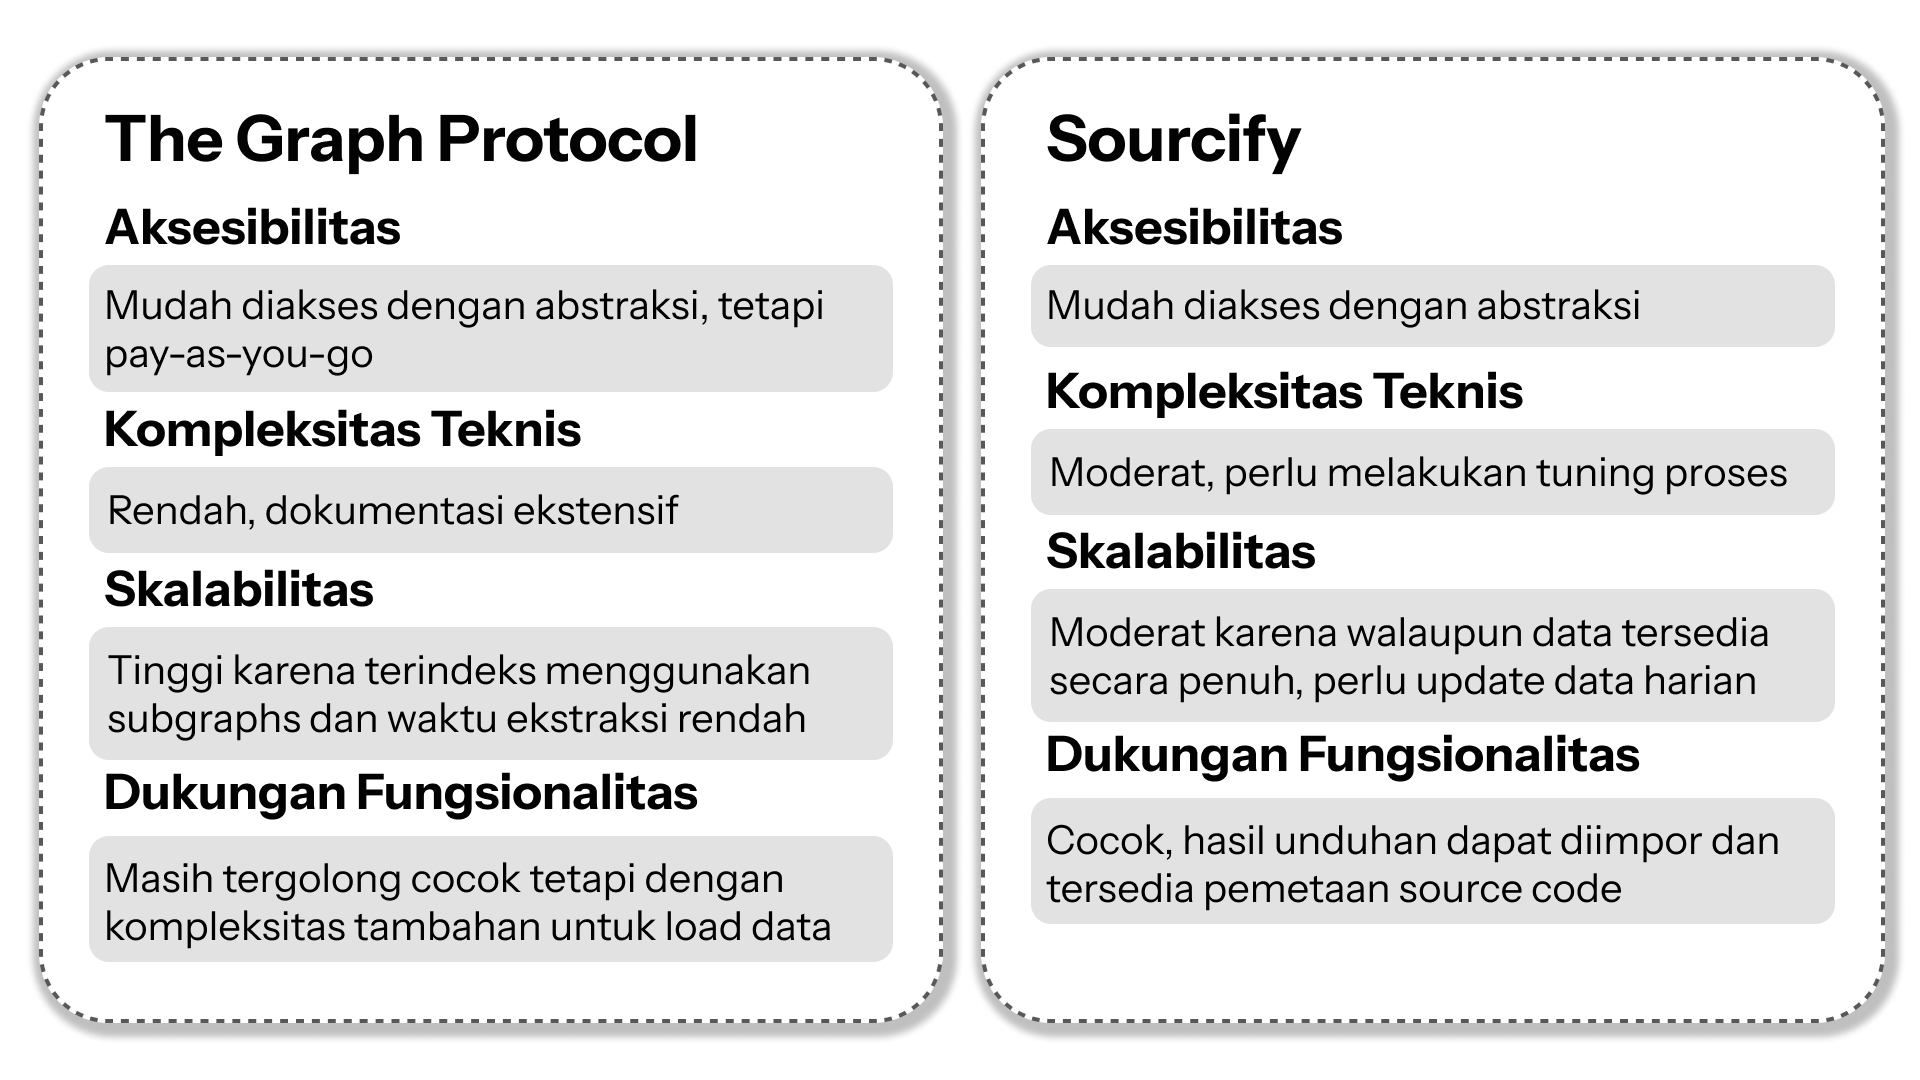
\includegraphics[width=0.9\textwidth]{resources/chapter-3/ekstraksi-3.png}
	\caption{Perbandingan alternatif ekstraksi data Smart Contracts dari Blockchain Ethereum}
	\label{image:perbandingan-ekstraksi-3}
\end{figure}

Kebutuhan pertama yang harus dipenuhi adalah ekstraksi data Smart Contracts dari Blockchain Ethereum. Proses ini mencakup pengambilan data terkait Smart Contracts, seperti ABI, bytecode, metadata, dan Verified \textit{source code}. Data ini akan digunakan untuk membangun basis data yang dapat di-query dan dianalisis lebih lanjut.

Dukungan fungsional yang diperlukan tidak hanya mencakup ekstraksi data, tetapi juga kemampuan memperoleh source code yang terverifikasi dan memetakan source code tersebut dengan deployment untuk analisis tanpa dekompilasi. Prioritas fungsionalnya adalah menghasilkan data dalam format siap pakai, memperoleh source code, dan mengaitkannya dengan deployment.

Gambar \ref{image:perbandingan-ekstraksi-1}, \ref{image:perbandingan-ekstraksi-2}, dan \ref{image:perbandingan-ekstraksi-3} menunjukkan rangkuman perbandingan berbagai alternatif ekstraksi data Smart Contracts dari Blockchain Ethereum. Secara rinci, berikut adalah analisis dari masing-masing alternatif:

\begin{enumerate}
	\item \textbf{eth2dgraph} \parencite{aimar2023extraction}: Riset ini unggul dalam mengekstrak ABI, bytecode, dan metadata yang dikonversi menjadi format graf. Implementasinya yang \textit{open source} menggunakan Rust untuk kinerja tinggi dan Dgraph untuk skalabilitas, sehingga memungkinkan query pada hubungan antar Smart Contracts di Ethereum. Pendekatan ini memerlukan \textit{node} Ethereum dan dasar pengetahuan mengenai Rust dan Dgraph. Selain ekstraksi cepat, eth2dgraph efektif dalam mengaitkan Smart Contracts Deployment dengan Verified \textit{source code} serta dapat diperluas untuk menambahkan aspek semantik.

	\item \textbf{Ethereum ETL} \parencite{ethereum_etl}: Ethereum ETL dikenal karena kemudahan penggunaan dan dokumentasinya yang lengkap, serta dukungan untuk data transaksi, blok, dan Smart Contracts. Meskipun demikian, ia tidak mendukung ekstraksi ABI, membutuhkan waktu lebih lama, dan memerlukan beberapa operasi tambahan untuk memperoleh data Smart Contracts. Hasil ekstraksinya cocok untuk basis data relasional, namun kurang ideal untuk sistem big data karena format data yang dihasilkan.

	\item \textbf{Etherscan API} \parencite{etherscan2024}: Dengan Etherscan API, pengguna dapat langsung mengekstrak data Smart Contracts beserta Verified \textit{source code} dari sumber yang terpercaya. Antarmukanya yang sederhana memudahkan akses, namun seluruh data bergantung pada Etherscan yang tersentralisasi. Batasan jumlah permintaan serta biaya penggunaan juga perlu diperhitungkan, terutama untuk ekstraksi data skala besar.

	\item \textbf{XBlock-ETH} \parencite{zheng2020xblock}: XBlock-ETH memungkinkan ekstraksi data tanpa memanfaatkan \textit{node} Ethereum, namun hasilnya disimpan dalam bentuk CSV yang memerlukan parsing tambahan dan tidak mendukung query atau indexing secara efisien. Selain itu, karena kode ekstraksinya tidak \textit{open source}, replikasi proses menjadi sulit meskipun pendekatannya cukup sederhana untuk digunakan.

	\item \textbf{The Graph Protocol} \parencite{TheGraphDocs}: The Graph menawarkan kemudahan penggunaan dengan query cepat dan infrastruktur yang terintegrasi dengan baik. Namun, model pembayaran \textit{pay-as-you-go} dapat membuat biaya ekstraksi data meningkat. Data JSON yang dihasilkan memerlukan konversi ulang ke format lain, meski flexibelnya memudahkan pengembangan lebih lanjut.

	\item \textbf{Sourcify} \parencite{sourcify_website}: Sourcify menyediakan antarmuka yang mudah untuk mengunduh dan memetakan hubungan antara \textit{source code} dan Deployment. Meskipun sudah tersedia abstraksi, ia tidak mendukung ekstraksi data kompleks seperti ABI dan bytecode. Proses pengunduhan berkala untuk memperbarui data masih perlu dioptimalkan agar lebih efisien, meskipun penggunaannya tergolong moderat.
\end{enumerate}


\subsubsection{Pemodelan, Penyimpanan, dan \textit{Indexing} Data Smart Contracts}

% jadi bahas alternatif dulu, misal yang terpilih eth2dgraph
% lalu bahas schema yang dipakainya gimana, yang base nya apa aja secara singkat, dan yang mau ditambahinnya apa, berdasarkan apa
% Jadiin dua subheading

\subsubsection{Klasifikasi Fungsional dan Semantik Smart Contracts}

\begin{figure}[ht]
	\centering
	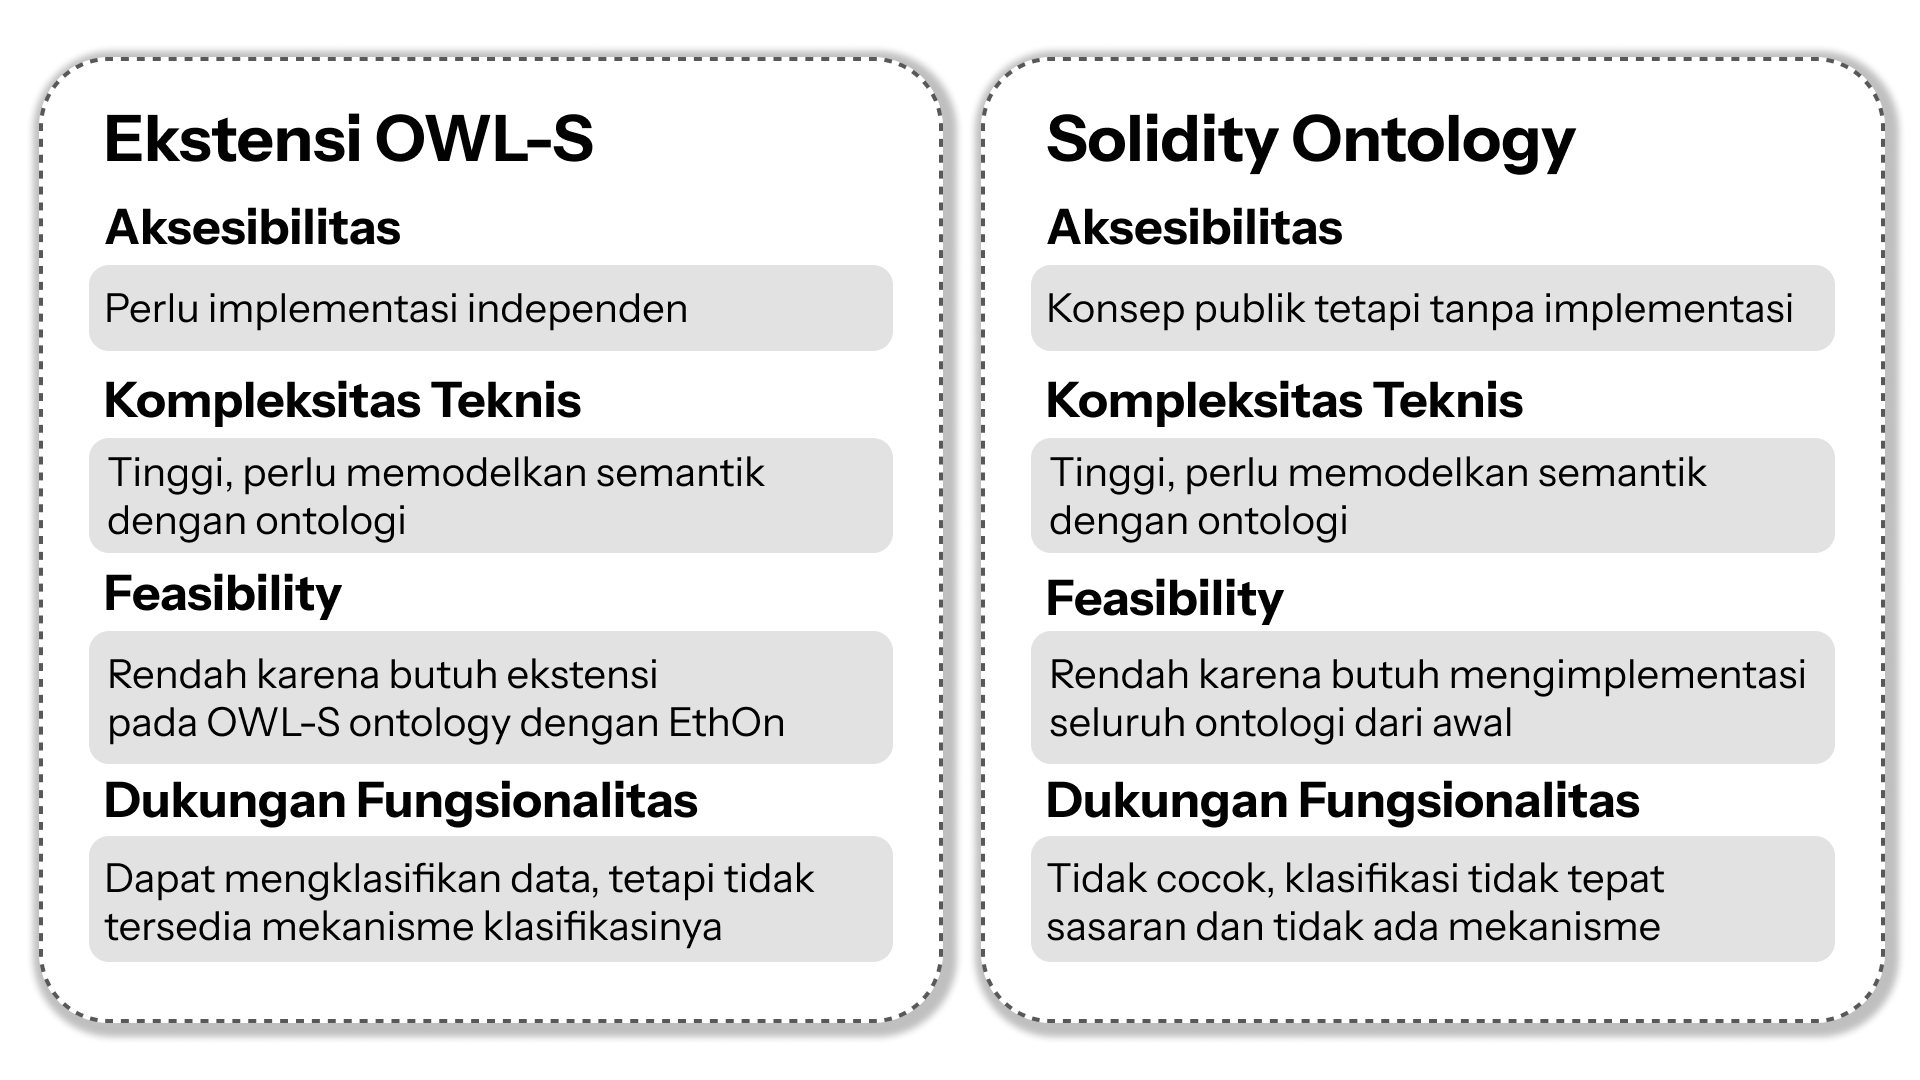
\includegraphics[width=0.9\textwidth]{resources/chapter-3/klasifikasi - 1.png}
	\caption{Perbandingan alternatif klasifikasi fungsional dan semantik Smart Contracts}
	\label{image:klasifikasi-1}
\end{figure}

\begin{figure}[ht]
	\centering
	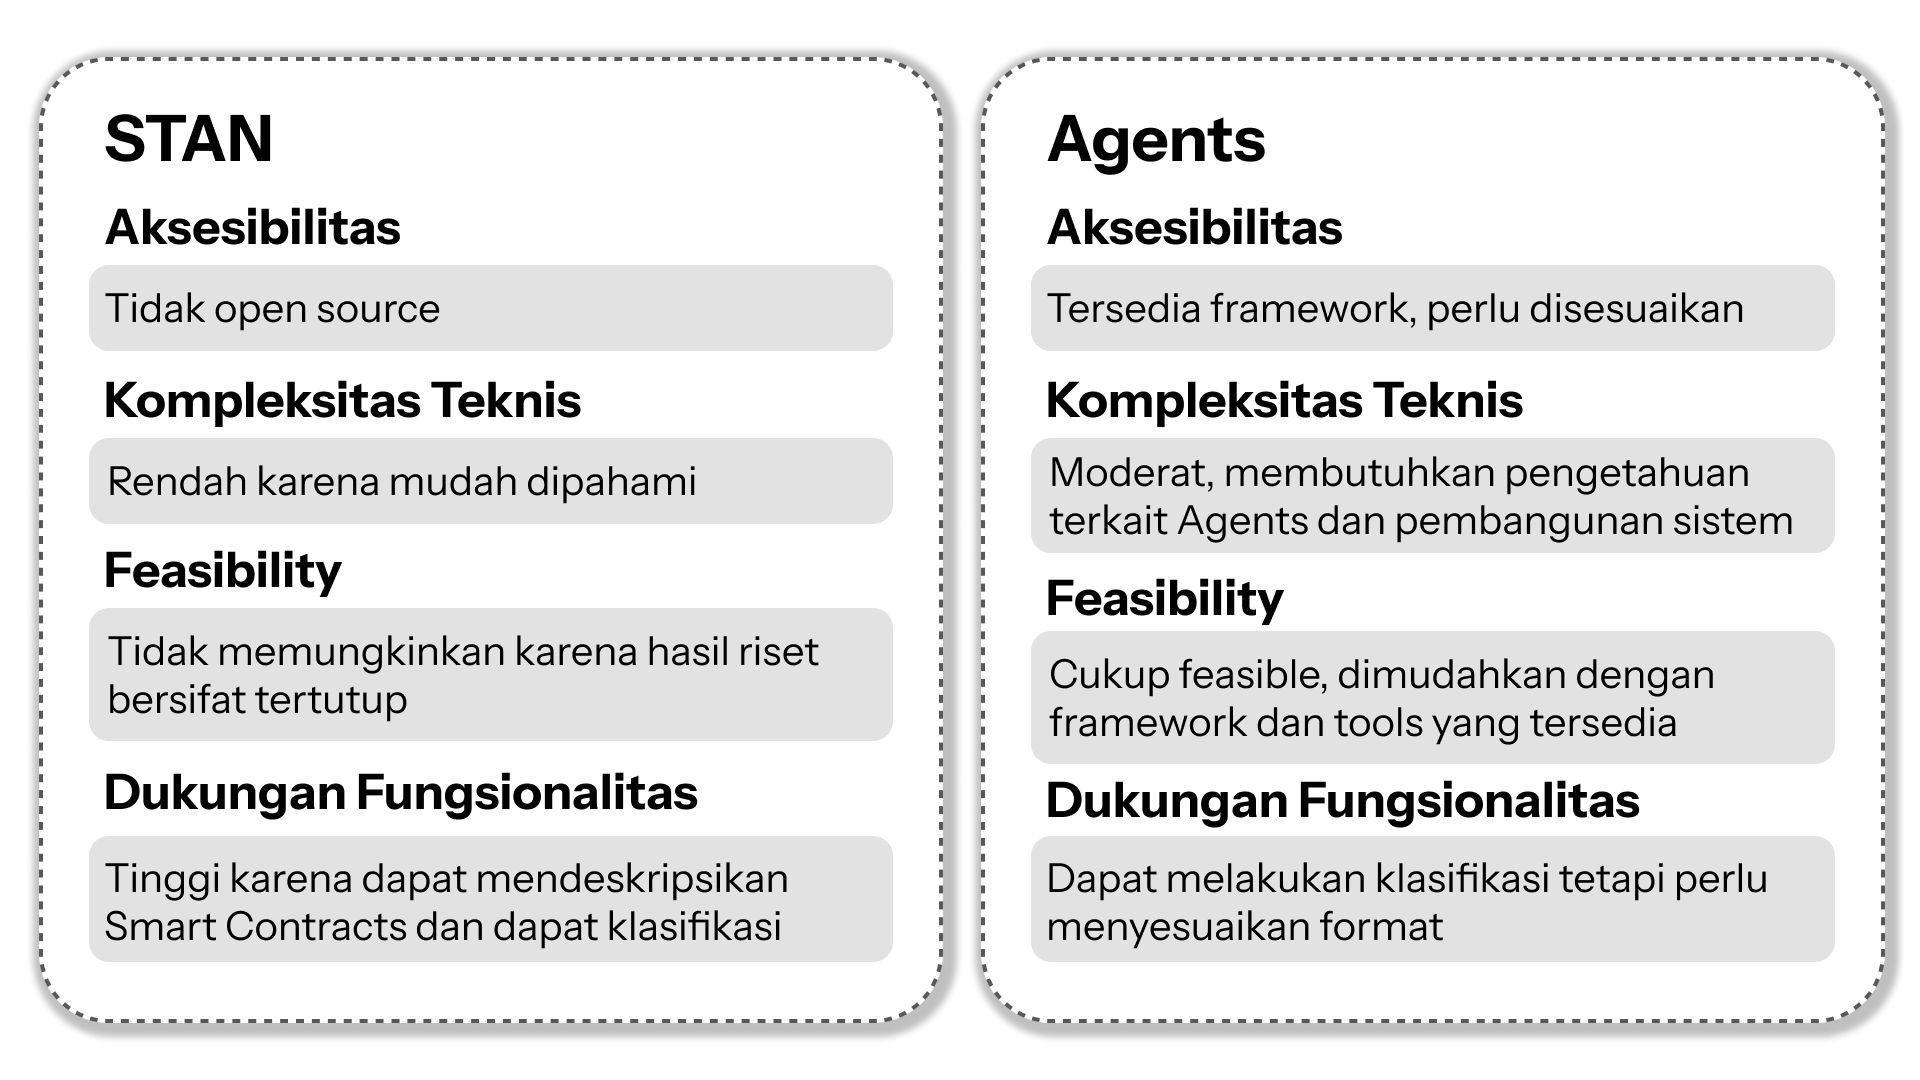
\includegraphics[width=0.9\textwidth]{resources/chapter-3/klasifikasi - 2.png}
	\caption{Perbandingan alternatif klasifikasi fungsional dan semantik Smart Contracts}
	\label{image:klasifikasi-2}
\end{figure}

\begin{figure}[ht]
	\centering
	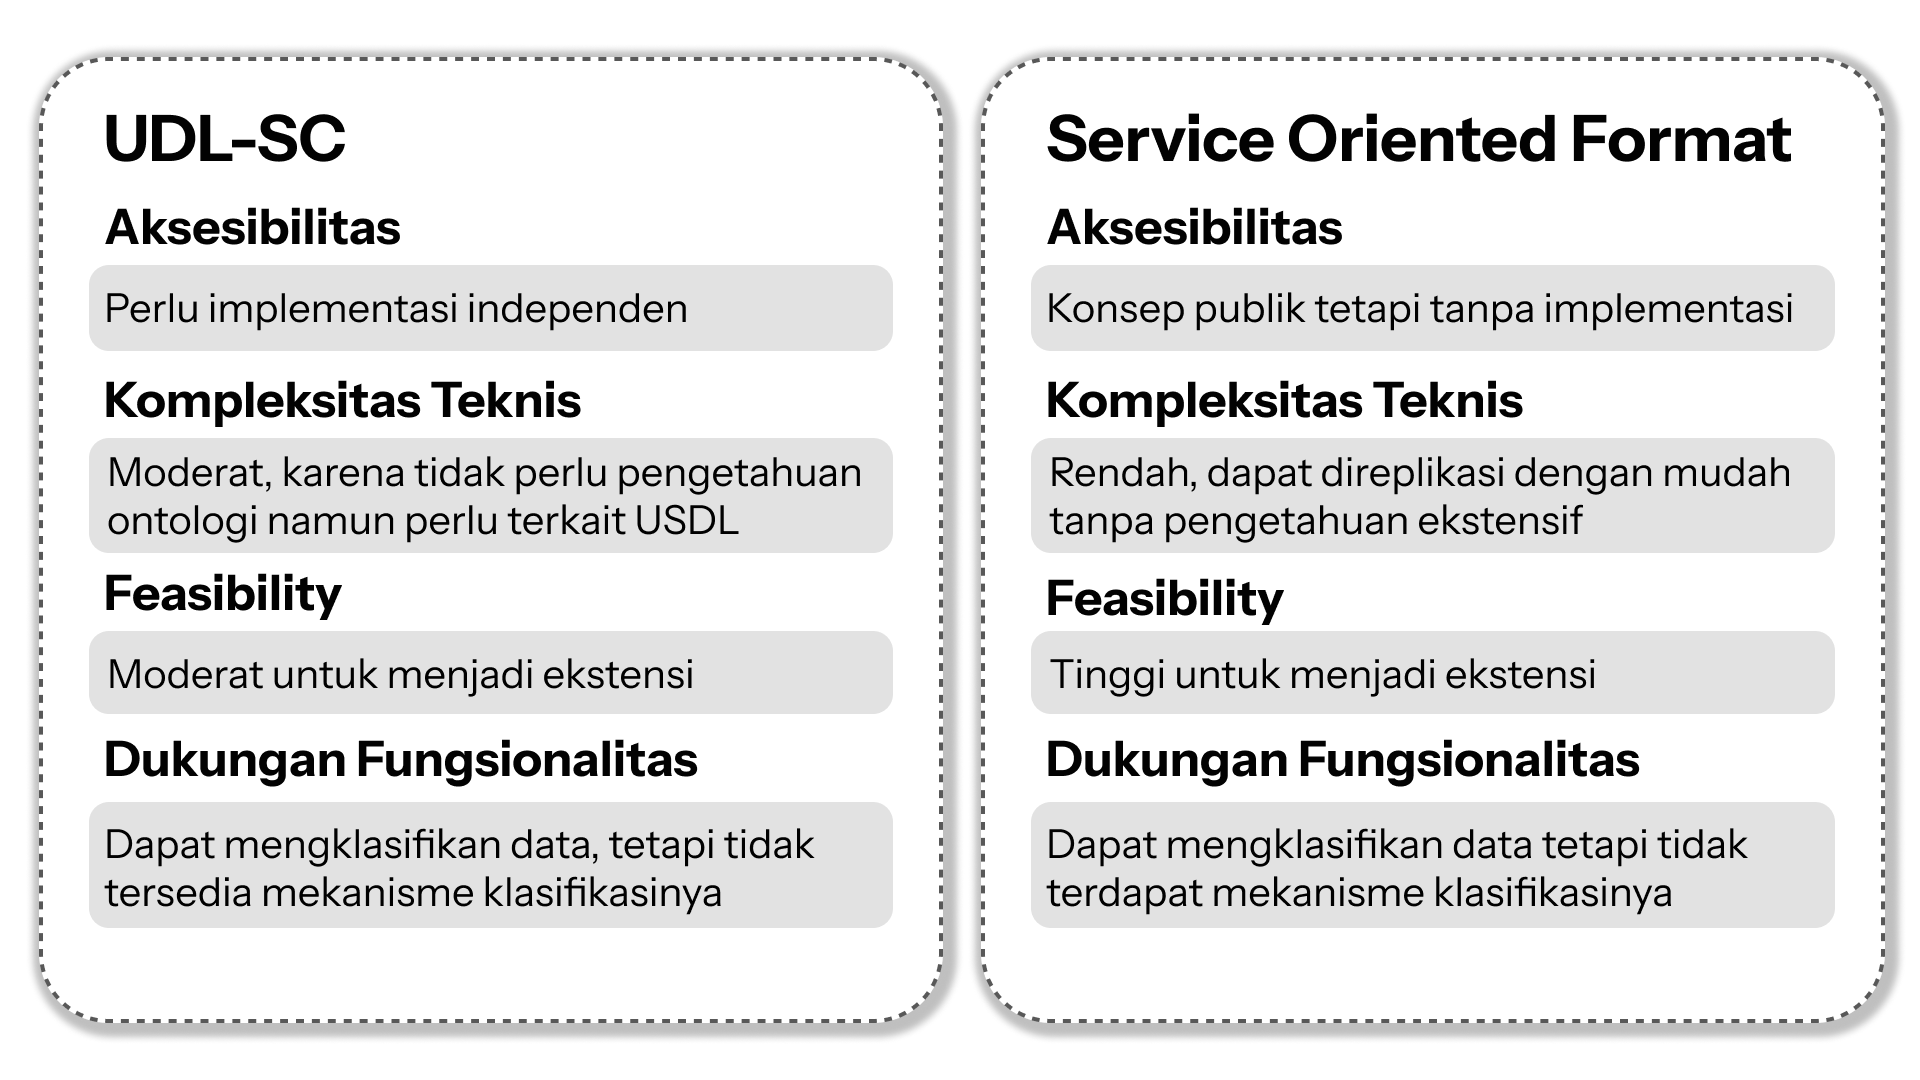
\includegraphics[width=0.9\textwidth]{resources/chapter-3/klasifikasi - 3.png}
	\caption{Perbandingan alternatif klasifikasi fungsional dan semantik Smart Contracts}
	\label{image:klasifikasi-3}
\end{figure}

\begin{figure}[ht]
	\centering
	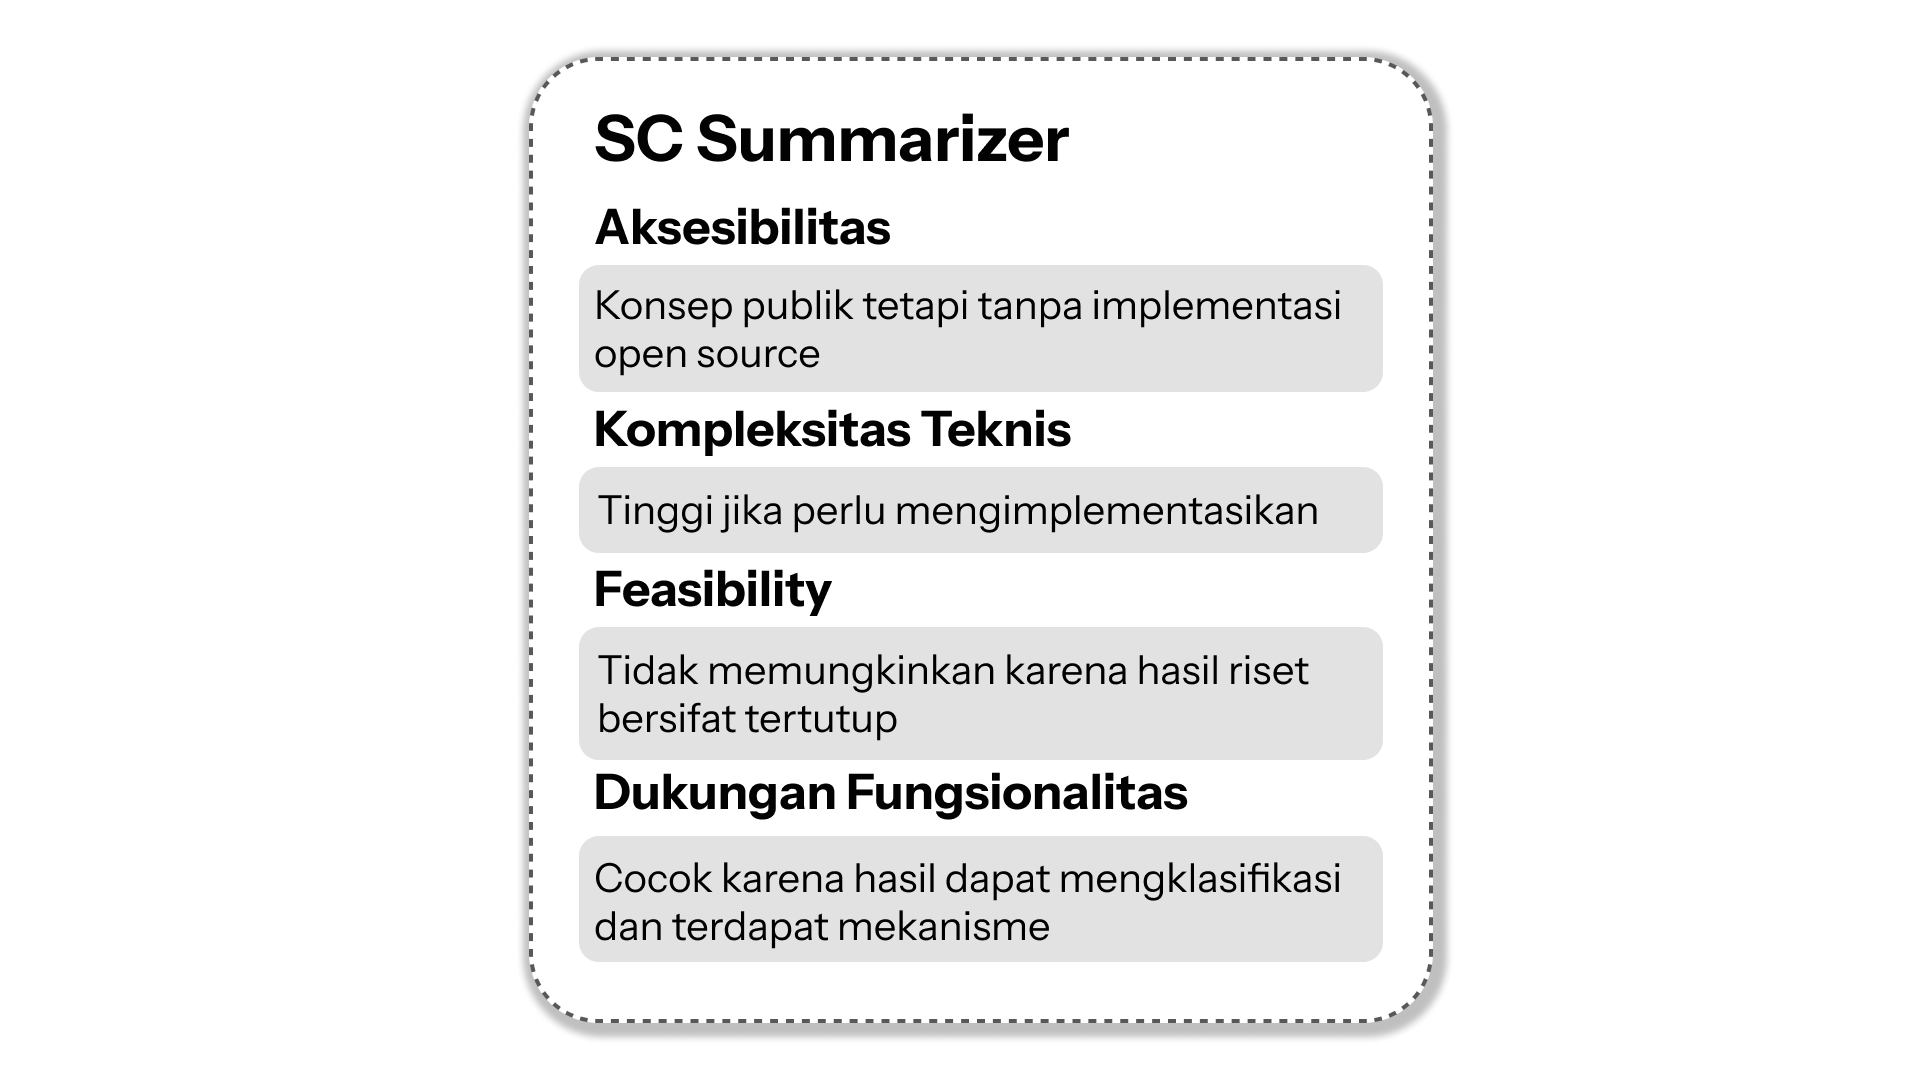
\includegraphics[width=0.9\textwidth]{resources/chapter-3/klasifikasi - 4.png}
	\caption{Perbandingan alternatif klasifikasi fungsional dan semantik Smart Contracts}
	\label{image:klasifikasi-4}
\end{figure}

Data yang sudah dimodelkan dan disimpan ke dalam sistem perlu dilakukan klasifikasi untuk memudahkan pencarian Smart Contracts berdasarkan fungsionalitas dan semantik. Terdapat berbagai alternatif untuk melakukan klasifikasi fungsional dan semantik Smart Contracts dengan berbagai pendekatan, baik dengan pemodelan ontologi, deskripsi fungsional, maupun format lainnya. Dukungan fungsional yang baik untuk klasifikasi adalah riset yang dapat melakukan klasifikasi pada data Smart Contracts dengan baik dan memberikan deskripsi atau hasil klasifikasi yang baik. Pada bagian ini, aspek skalabilitas digantikan dengan aspek \textit{feasibility}.

Gambar \ref{image:klasifikasi-1}, \ref{image:klasifikasi-2}, \ref{image:klasifikasi-3}, dan \ref{image:klasifikasi-4} menunjukkan rangkuman perbandingan berbagai alternatif klasifikasi fungsional dan semantik Smart Contracts. Secara rinci, berikut adalah analisis dari masing-masing alternatif:

\begin{enumerate}
	\item \textbf{Semantic Smart Contracts for Blockchain-based Services in the Internet of Things} \parencite{baqa2019semantic} (Bagian \ref{subsec:semantic-smart-contract-iot}): Riset ini menggunakan ekstensi pada OWL-S Service Ontology untuk melakukan klasifikasi Smart Contracts berdasarkan semantik dan fungsionalitas. Keunggulannya adalah penggunaan ontologi yang dapat di-\textit{extend} untuk menambahkan terminologi yang \textit{domain specific}. Secara aksesibilitas, riset ini bersifat \textit{public}, namun tidak memiliki implementasi \textit{open source}. Selain itu, riset ini terbatas pada \textit{scope} Internet-of-Things. Secara kompleksitas, riset ini tergolong tinggi karena memerlukan pemahaman yang mendalam tentang ontologi dan pemodelan semantik. Dalam hal dukungan fungsional, riset ini dapat memberikan deskripsi yang baik, tetapi tidak terdapat mekanisme untuk mengklasifikasikan data dengan baik.

	\item \textbf{Ontological Modeling of Smart Contracts in Solidity} \parencite{cano2021toward} (Bagian \ref{subsec:solidity-ontology}): Riset ini menerapkan ontologi pada bahasa pemrograman Solidity. Ontologi ini digunakan untuk mendeskripsikan elemen-elemen dalam Smart Contracts, seperti fungsi, variabel, dan struktur data. Secara aksesibilitas, riset ini bersifat publik, dengan ontologi yang dihasilkan dapat diterapkan. Namun, implementasi ontologi pada riset ini terbatas pada sintaks dan semantik dari kode bahasa pemrograman Solidity sendiri dibandingkan Smart Contracts secara keseluruhan. Secara kompleksitas, riset ini tergolong tinggi karena memerlukan pemahaman yang mendalam tentang ontologi dan pemodelan semantik, dan memerlukan proses klasifikasi yang ekstensif untuk memetakan data dengan ontologi yang dihasilkan. Dalam hal dukungan fungsional, riset ini tidak sesuai dengan kebutuhan sistem, yaitu memodelkan fungsionalitas dari Smart Contract, bukan aspek sintaks bahasa pemrograman Soliditynya, dan tidak terdapat mekanisme untuk mengklasifikasikan data dengan baik.

	\item \textbf{STAN} \parencite{stan} (Bagian \ref{subsec:stan}): STAN adalah sebuah sistem untuk memberikan deskripsi terhadap bytecodes dari Smart Contracts. Secara aksesibilitas, STAN tidak bersifat \textit{open source}, sehingga tidak tersedia implementasinya untuk melakukan replikasi. Secara kompleksitas, STAN tergolong rendah karena abstraksi yang sudah diberikan untuk menghasilkan deskripsi. Riset STAN ini juga belum menginkorporasikan teknologi seperti Artificial Intelligence (AI) untuk melakukan klasifikasi. Dalam hal dukungan fungsional, STAN dapat membantu mengklasifikasikan Smart Contracts berdasarkan deskripsi yang dihasilkan.

	% \item \textbf{Agents} (Bagian \ref{sec:agents}): Alternatif untuk melakukan klasifikasi Smart Contracts adalah menggunakan AI Agents yang dapat melakukan dekomposisi tasks yang kompleks menjadi sub-tasks yang lebih sederhana. Dengan menggunakan AI Agents, klasifikasi Smart Contracts dapat dilakukan dengan lebih menyeluruh dan efisien karena dapat memperhitungkan berbagai aspek yang ada pada Smart Contracts. Secara aksesibilitas, sudah banyak \textit{framework} dan \textit{tools} yang tersedia untuk membangun sebuah sistem berbasis AI Agents (Agentic AI). Namun, perlu dilakukan pembangunan secara independen karena tidak ada sistem yang secara langsung memberikan fungsionalitas yang sesuai. Secara kompleksitas, penggunaan AI Agents tergolong moderat karena memerlukan pengetahuan terkait AI dan membuat sistem berbasis AI Agents. Secara \textit{feasibility}, pembangunan sistem berbasis agents cukup \textit{feasible} dengan penggunaan \textit{framework} dan \textit{tools} yang baik. Dukungan fungsional yang diberikan oleh sistem dengan AI Agents tergolong baik karena dapat disesuaikan dan melakukan pekerjaan kompleks secara otonom, tetapi perlu menggunakan format yang disesuaikan untuk mendeskripsikan data.
	      % menggunakan agents yang dimasukkin source code, dengan break down step by step

	\item \textbf{LLM Classification} (Bagian \ref{sec:llms}): Penggunaan LLM untuk melakukan klasifikasi Smart Contracts dengan menghasilkan deskripsi dan mengklasifikasikan berdasarkan deskripsi yang dihasilkan. Dengan memanfaatkan kemampuan LLM dalam memahami konteks dan semantik, diharapkan klasifikasi dapat dilakukan dengan lebih akurat dan efisien. Secara aksesibilitas, LLMs seperti GPT-4 dan Llama-3 sudah tersedia untuk digunakan, baik melalui API maupun model yang dapat diunduh. Secara kompleksitas, penggunaan LLMs tergolong rendah karena hanya memerlukan pengetahuan dasar tentang pemrograman dan penggunaan API. Secara \textit{feasibility}, sistem ini \textit{feasible} untuk diimplementasikan dengan infrastruktur yang ada. Dalam hal dukungan fungsional, LLMs dapat memberikan deskripsi yang baik dan melakukan klasifikasi Smart Contracts dengan baik, tetapi perlu diperhatikan bahwa LLMs tidak selalu memberikan hasil yang konsisten.

	\item \textbf{Uniform Description Language for Smart Contracts} \parencite{udlsc} (Bagian \ref{subsec:uniform-description-language}): Riset ini mengusulkan sebuah bahasa deskripsi ekstensi dari USDL untuk Smart Contracts. Secara aksesibilitas, hasil dari riset ini bersifat \textit{public}, namun perlu melakukan replikasi untuk mendapatkan hasil yang didapatkan dari riset. Secara kompleksitas, riset ini tergolong moderat karena walaupun tidak memerlukan pengetahuan yang mendalam terkait ontologi, perlu memahami terkait USDL dan implementasi ekstensi dari USDL. Secara skalabilitas, riset ini tergolong baik karena dapat digunakan sebagai ekstensi data tanpa masalah. Dalam hal dukungan fungsional, riset ini kurang baik karena tidak terdapat mekanisme untuk mengklasifikasikan data dengan baik, tetapi dapat digunakan untuk mendeskripsikan data Smart Contracts dengan baik.

	\item \textbf{Service Oriented Format Descriptor} \parencite{guida2019supporting} (Bagian \ref{subsec:supporting-reuse-smart-contracts}): Riset ini mengusulkan sebuah format deskripsi untuk Smart Contracts dengan pendekatan Service. Riset ini juga mengusulkan sebuah Service Registry dan Contract Editor berbasis visual yang mengkomplemen format deskripsi yang diusulkan. Format deskripsi ini dapat digunakan dan digabungkan dengan sistem lain, sedangkan Service Registry dan Contract Editor kurang fleksibel untuk diintegrasikan dengan sistem lain. Secara aksesibilitas, hasil dari riset ini bersifat \textit{public} dan \textit{open source}, sehingga dapat digunakan untuk melakukan replikasi. Secara kompleksitas, format yang dihasilkan oleh riset ini tergolong rendah karena tidak memerlukan pengetahuan yang mendalam dan dapat langsung dijadikan ekstensi ke format lain. Dalam hal dukungan fungsional, riset ini dapat mengakomodasi deskripsi Smart Contracts dengan baik, tetapi tidak ada mekanisme untuk melakukan klasifikasi data dengan baik.

	\item \textbf{Smart Contract Summarizer} \parencite{zhang2021smart} (Bagian \ref{subsec:smart-contract-solidity-summary}): Riset ini mengusulkan sebuah sistem untuk menghasilkan ringkasan dan anotasi dari Smart Contracts, terutama dalam bahasa Solidity. Sistem ini menggunakan teknik NLG (Natural Language Generation) dengan pendekatan berbasis \textit{transformer} untuk menghasilkan ringkasan yang lebih baik dibandingkan dengan metode berbasis template sebelumnya. Secara aksesibilitas, konsep dari riset ini bersifat \textit{public}, namun tidak memiliki implementasi \textit{open source}. Secara kompleksitas, jika perlu mengimplementasikan dari awal, riset ini tergolong tinggi karena memerlukan pengetahuan yang mendalam terkait NLP dan pemodelan semantik. Secara skalabilitas, sistem ini tidak diketahui untuk kinerja menangani data yang banyak. Dalam hal dukungan fungsional, riset ini dapat membantu mengklasifikasikan Smart Contracts berdasarkan ringkasan yang dihasilkan dengan mekanisme yang digunakan.

\end{enumerate}


\subsubsection{Pencarian dan Rekomendasi Smart Contracts}

% ini LLM, terus pake langchain?? (iya si harusnya (recheck obsidian pls))

\subsubsection{Interaksi Pengguna dengan Sistem}


\subsubsection{Kesimpulan Pemilihan Alternatif}

\begin{figure}[ht]
	\centering
	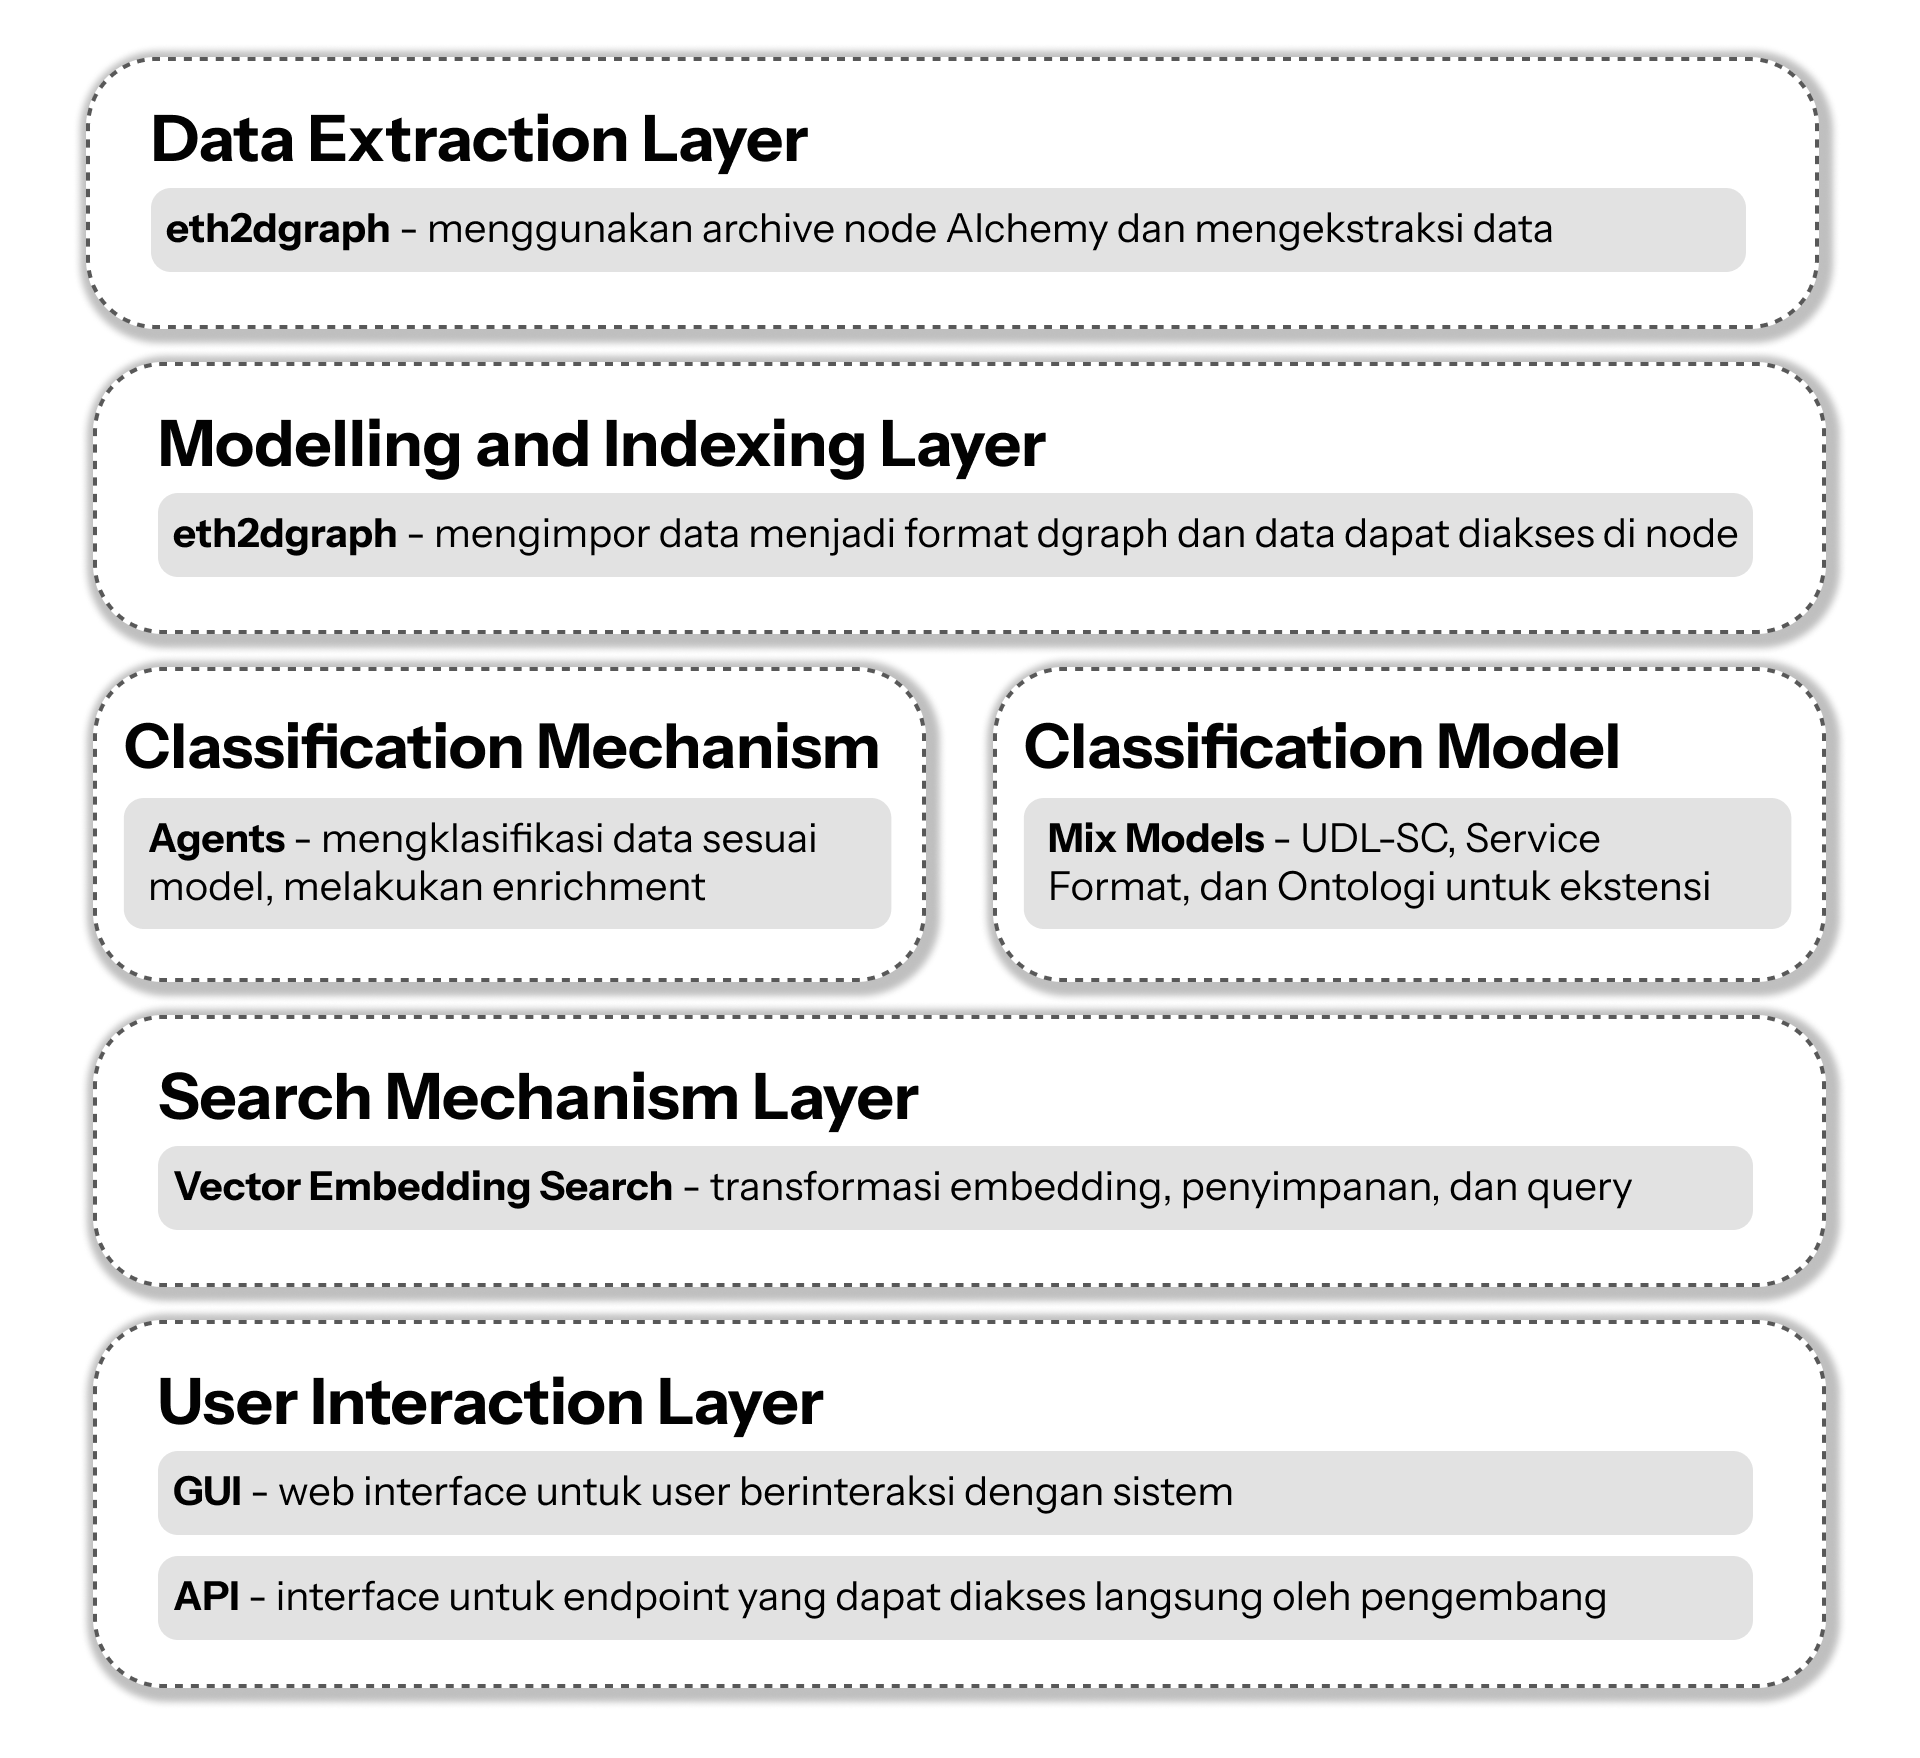
\includegraphics[width=0.7\textwidth]{resources/chapter-3/hasil-pemilihan.png}
	\caption{Kesimpulan pemilihan alternatif}
	\label{image:layer-architecture}
\end{figure}

Berdasarkan analisis dari alternatif-alternatif yang dibahas pada bagian \ref{subsec:analisis-alternatif-solusi}, dapat disimpulkan bahwa alternatif yang dipilih untuk membangun sistem adalah sebagai berikut:

\begin{enumerate}
	\item \textbf{Ekstraksi data Smart Contracts dari Blockchain Ethereum}: Alternatif yang dipilih adalah \textit{eth2dgraph} \parencite{aimar2023extraction}, karena memiliki aksesibilitas yang baik, bersifat \textit{open source}, memiliki kecepatan ekstraksi yang tinggi, dan juga menyediakan infrastruktur lengkap sampai pada penyimpanan data dalam format Distributed Graph Database.
	\item \textbf{Pemodelan, penyimpanan, dan \textit{indexing} data Smart Contracts}: Alternatif yang dipilih adalah \textit{eth2dgraph} \parencite{aimar2023extraction}, karena memiliki kemampuan skalabilitas tinggi dan dapat melakukan query dengan efisien. Selain itu, Dgraph juga memiliki kemampuan untuk melakukan \textit{indexing} data dengan baik.
	\item \textbf{Klasifikasi fungsional dan semantik Smart Contracts}: Alternatif yang dipilih untuk mekanisme klasifikasi adalah LLM Classification, karena memliki kemampuan kustomisasi yang baik untuk mendeskripsikan dan mengklasifikasi Smart Contracts. Model yang akan digunakan adalah model tekstual, yaitu penjelasan fungsionalitas Smart Contracts dalam bahasa alami, dengan kombinasi dengan konsep ontologi dalam bentuk metadata untuk pengklasifikasian. Metadata dengan konsep ontologi ini akan membuat atribut data lebih mudah untuk diekstrak menjadi sebuah ontologi.
	\item \textbf{Pencarian dan rekomendasi Smart Contracts}: Alternatif yang dipilih untuk mekanisme pencarian awal adalah alternatif Vector Embedding Search, karena simplisitas yang ditawarkan dan tidak ada redundansi \textit{layer}. Alternatif yang dapat dikonsiderasikan untuk pengembangan berikutnya, terutama jika dikembangkan sebuah fitur untuk berinteraksi dengan sistem yang lebih kompleks adalah alternatif \textit{Retrieval-Augmented Generation (RAG)}, karena dapat mengakomodasi interaksi yang lebih kompleks.
	\item \textbf{Interaksi pengguna dengan sistem}: API dan GUI akan diimplementasikan untuk interaksi pengguna dengan sistem karena dapat memberikan fleksibilitas dan kemudahan bagi pengguna. Sehingga, pengguna dapat melakukan pencarian Smart Contracts dengan cara yang sesuai dengan kebutuhan mereka.
\end{enumerate}

% Untuk mengatasi permasalahan pemilihan Smart Contracts yang tepat dan mengurangi redundansi Smart Contracts di Blockchain, solusi yang diusulkan adalah sebuah sistem pencarian Smart Contracts yang dapat memberikan hasil berdasarkan fungsionalitas Smart Contracts. Sistem akan dibangun dengan memanfaatkan berbagai teknologi dan riset yang sudah ada, yang melakukan \textit{indexing} maupun modeling yang menjadikan Smart Contracts \textit{discoverable} untuk mengefisiensikan pengembangan.

% Beberapa riset yang dilakukan peninjauan untuk digunakan sebagai basis adalah riset oleh \cite{third2017linked}, \cite{aimar2023extraction}, \cite{baqa2019semantic}, \cite{cano2021toward}. Peninjauan didasari dengan beberapa aspek yaitu aksesibilitas dari hasil riset, kompleksitas teknis, skalabilitas, dan dukungan fungsional untuk mencapai tujuan utama.

% % Masukin diagram yang dibuat di ppt

% % preliminary analysis

% % gambaran solusi

% % menjelaskan secara lebih detail latar belakang dan masalah yang menjadi dasar munculnya topik TA ini, intinya kita coba lihat & analisis gapnya 
% % gap analysis
% % kaitan antara sistem yang dikembangkan dengan yang terkait -> apa kelebihannya? atau apa kekurangan dari aplikasi lain? emang belum terpenuhi? apa yang belum terpenuhi?
% % posisi sistem yang dikembangkan terhadap sistem yang lebih besar

% % PLACEHOLDER
% \subsubsection{Semantic Indexing with Linked Data \parencite{third2017linked}}

% Riset ini menerapkan indeks semantik pada data Blockchain menggunakan Linked Data dengan keunggulan penggunaan ontology BLONDiE dan MSM untuk mendeskripsikan semantik Smart Contracts dan fokus pada aspek \textit{discoverability}. Secara aksesibilitas, konsep riset ini \textit{public}, namun tanpa implementasi \textit{open source}. Implementasinya kompleks karena memerlukan pemetaan ontology ekstensif dan RDF triple generation, tanpa dukungan \textit{tools} atau \textit{framework}. Skalabilitas riset ini terbatas karena bergantung pada RDF-based Linked Data, yang kurang cocok untuk data Blockchain besar.

% \subsubsection{eth2dgraph \parencite{aimar2023extraction}}

% Riset ini berfokus pada ekstraksi, \textit{indexing}, dan penyimpanan data Ethereum berbasis Distributed Graph. Keunggulannya adalah penggunaan ekstraksi ABI, bytecode, dan metadata yang dapat diubah menjadi format berbasis graf, serta implementasinya yang \textit{open source} dan \textit{public}. Menggunakan Rust untuk performa tinggi dan Dgraph untuk skalabilitas, riset ini dapat melakukan query pada hubungan Smart Contracts di Ethereum. Kompleksitasnya moderat karena memerlukan pengetahuan dasar tentang Rust dan Dgraph, namun dapat diperluas untuk menambahkan aspek semantik. Skalabilitasnya tinggi berkat kinerja Dgraph.

% \subsubsection{Alternatif Lainnya}

% Kedua riset alternatif lainnya oleh \cite{baqa2019semantic} dan \cite{cano2021toward} tidak dapat dipilih karena \textit{domain} yang terlalu spesifik, ditambah dengan implementasi yang tidak bersifat \textit{open source} dan \textit{public}.

% \subsubsection{Hasil Analisis}

% Setelah melakukan analisis dari alternatif yang ada, diputuskan untuk menggunakan riset oleh \cite{aimar2023extraction}, karena memiliki implementasi yang \textit{open source}, yang mempermudah ekstraksi dan \textit{indexing} data menjadi Graph Database, sehingga tidak perlu membuat RDF Triples ada model ontology dari awal. Distributed Graph Database juga memiliki skalabilitas yang baik untuk data yang banyak pada Blockchain Ethereum. eth2dgraph juga memiliki kemampuan ekstensibilitas yang baik dalam \textit{domain} yang lebih umum, sehingga lebih mudah diimplementasikan sebagai fondasi dari sistem keseluruhan. 

% \subsubsection{Rancangan Solusi}

% Dengan penggunaan eth2dgraph sebagai fondasi dari sistem pencarian Smart Contract, berikut merupakan ajuan rancangan dari sistem:

% \begin{enumerate}
%   \item Layer 1: Blockchain Data Extraction (eth2dgraph) \newline Ekstraksi data Blockchain Ethereum menjadi Dgraph
%   \item Layer 2: Semantic Indexing and Enrichment \newline \textit{Mapping} data hasil ekstraksi kepada sebuah ontology seperti BLONDiE atau EthOn, pelabelan fungsional Smart Contracts, dan Version Control
%   \item Layer 3: Query and Discovery System \newline Sebuah Search Engine menggunakan GraphQL Queries diatas Dgraph Database yang memperkenalkan pencarian berbasis semantik
%   \item Layer 4: User Interaction Layer \newline Sebuah \textit{dashboard} atau API untuk pengembang melakukan pencarian Smart Contracts berdasarkan fungsionalitas, metadata, atau relasi, membandingkan Smart Contracts yang serupa, dan melakukan \textit{export} atau \textit{reuse} dari Smart Contract 
% \end{enumerate}
